\savestack{\nnoutputone}{\hspace{-0.1in}
\tikzstyle{input_neuron}=[circle,draw=red!50,fill=red!10,thick,minimum size=5mm]
\tikzstyle{hidden_neuron}=[circle,draw=blue!50,fill=cyan!10,thick,minimum size=6mm]
\tikzstyle{output_neuron}=[circle,draw=green!50,fill=green!10,thick,minimum size=6mm]
\tikzstyle{bias_neuron}=[circle,draw=red!50,fill=red!10,thick,minimum size=2mm]
\tikzstyle{bias_hidden_neuron}=[circle,draw=blue!50,fill=cyan!10,thick,minimum size=2mm]

\tikzstyle{input}=[circle,draw=black!50,fill=black!20,thick,minimum size=6mm]

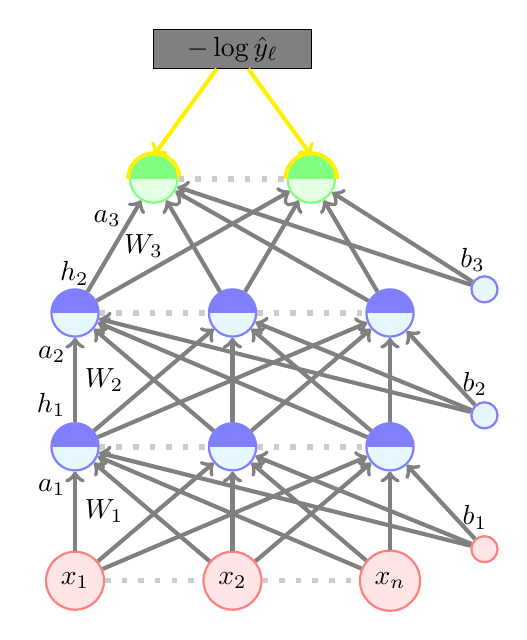
\begin{tikzpicture}


	\node [input_neuron] (neuron01) at (0,0) {$x_1$};
	\node [input_neuron] (neuron02) at (2,0){$x_2$};
	\node [input_neuron] (neuron03) at (4,0) {$x_n$};

	\node [bias_neuron] (neuron04) at (5.2,0.4) {};


	\node [hidden_neuron] (neuron11) at (0,1.7)  {};
	\node [hidden_neuron] (neuron12) at (2,1.7)  {};
	\node [hidden_neuron] (neuron13) at (4,1.7)  {};

	\node [bias_hidden_neuron] (neuron14) at (5.2,2.1) {};

	\begin{scope}
		\path[clip] (0,1.7) circle (3mm);
		\path[fill=blue!50] (-0.4,1.7) rectangle (0.3,2);
	\end{scope}
	\begin{scope}
		\path[clip] (2,1.7) circle (3mm);
		\path[fill=blue!50] (1.6,1.7) rectangle (2.3,2);
	\end{scope}
	\begin{scope}
		\path[clip] (4,1.7) circle (3mm);
		\path[fill=blue!50] (3.6,1.7) rectangle (4.3,2);
	\end{scope}


	\node [hidden_neuron] (neuron21) at (0,3.4)  {};
	\node [hidden_neuron] (neuron22) at (2,3.4)  {};
	\node [hidden_neuron] (neuron23) at (4,3.4)  {};

	\node [bias_hidden_neuron] (neuron24) at (5.2,3.7) {};


	\begin{scope}
		\path[clip] (0,3.4) circle (3mm);
		\path[fill=blue!50] (-0.4,3.4) rectangle (0.4,3.7);
	\end{scope}
	\begin{scope}
		\path[clip] (2,3.4) circle (3mm);
		\path[fill=blue!50] (1.6,3.4) rectangle (2.4,3.7);
	\end{scope}
	\begin{scope}
		\path[clip] (4,3.4) circle (3mm);
		\path[fill=blue!50] (3.6,3.4) rectangle (4.4,3.7);
	\end{scope}


	\node [output_neuron] (neuron31) at (1,5.1)  {};
	\node [output_neuron] (neuron32) at (3,5.1)  {};
	\draw [fill=gray] (1, 7) rectangle (3, 6.5) node[pos=0.5] {$-\log\hat{y}_\ell$};
	\draw [yellow,line width=1.5pt,  ->] (1.8, 6.5) -- (1, 5.4);
	\draw [yellow, line width=1.5pt, ->]  (2.2, 6.5) -- (3, 5.4);
	\draw [yellow, line width = 3] (1.3,5.1) arc (0:180:3mm) {};
	\draw [yellow, line width = 3] (3.3,5.1) arc (0:180:3mm) {};

	\begin{scope}
		\path[clip] (1,5.1) circle (3mm);
		\path[fill=green!50] (0.6,5.1) rectangle (1.3,5.4);
	\end{scope}
	\begin{scope}
		\path[clip] (3,5.1) circle (3mm);
		\path[fill=green!50] (2.6,5.1) rectangle (3.3,5.4);
	\end{scope}

	\draw[white,->] (neuron01) -- (neuron11) node[black,pos=.5,right]  {$W_{1}$} node[black,pos=0.8,left] {$a_{1}$};

	\draw[white,->] (neuron11) -- (neuron21) node[black,pos=.5,right] {$W_{2}$} node[black,pos=0.8,left] {$a_{2}$} node[black,pos=.2,left] {$h_{1}$};
	\draw[white,->] (neuron21) -- (neuron31) node[black,pos=.5,right] {$W_{3}$} node[black,pos=0.8,left] {$a_{3}$} node[black,pos=.2,left] {$h_{2}$};

	\draw[white,->] (neuron04) -- (neuron13) node[black,pos=0,right,above] {$b_1$};

	\draw[white,->] (neuron14) -- (neuron23) node[black,pos=0,right,above] {$b_2$};

	\draw[white,->] (neuron24) -- (neuron32) node[black,pos=0,right,above] {$b_3$};

	\draw[black!20,line width=2pt,loosely dotted] (neuron01) -- (neuron02);
	\draw[black!20,line width=2pt,loosely dotted] (neuron02) -- (neuron03);
	\draw[black!20,line width=2pt,loosely dotted] (neuron11) -- (neuron12);
	\draw[black!20,line width=2pt,loosely dotted] (neuron12) -- (neuron13);
	\draw[black!20,line width=2pt,loosely dotted] (neuron21) -- (neuron22);
	\draw[black!20,line width=2pt,loosely dotted] (neuron22) -- (neuron23);
	\draw[black!20,line width=2pt,loosely dotted] (neuron31) -- (neuron32);


	\foreach \from in {neuron01,neuron02,neuron03,neuron04}
	\foreach \to in {neuron11,neuron12,neuron13}
	\draw [black!50,line width=1.5pt,->] (\from) -- (\to);

	\foreach \from in {neuron11,neuron12,neuron13,neuron14}
	\foreach \to in {neuron21,neuron22,neuron23}
	\draw [black!50,line width=1.5pt,->] (\from) -- (\to);

	\foreach \from in {neuron21,neuron22,neuron23,neuron24}
	\foreach \to in {neuron31,neuron32}
	\draw [black!50,line width=1.5pt,->] (\from) -- (\to);


\end{tikzpicture}
}
\savestack{\nnoutputtwo}{\hspace{-0.1in}
\tikzstyle{input_neuron}=[circle,draw=red!50,fill=red!10,thick,minimum size=5mm]
\tikzstyle{hidden_neuron}=[circle,draw=blue!50,fill=cyan!10,thick,minimum size=6mm]
\tikzstyle{output_neuron}=[circle,draw=green!50,fill=green!10,thick,minimum size=6mm]
\tikzstyle{bias_neuron}=[circle,draw=red!50,fill=red!10,thick,minimum size=2mm]
\tikzstyle{bias_hidden_neuron}=[circle,draw=blue!50,fill=cyan!10,thick,minimum size=2mm]

\tikzstyle{input}=[circle,draw=black!50,fill=black!20,thick,minimum size=6mm]

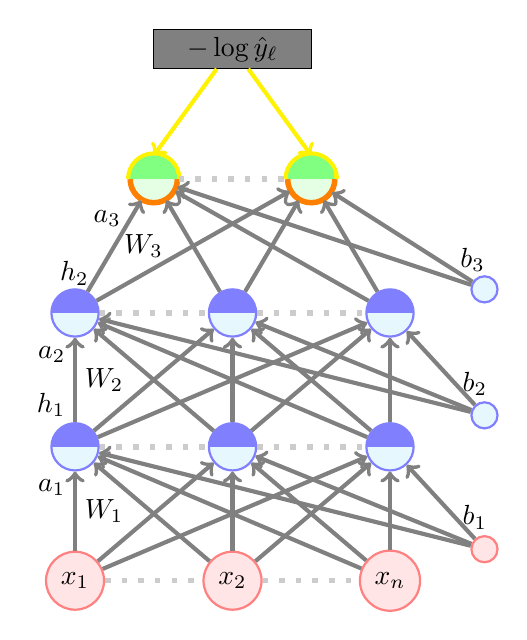
\begin{tikzpicture}


	\node [input_neuron] (neuron01) at (0,0) {$x_1$};
	\node [input_neuron] (neuron02) at (2,0){$x_2$};
	\node [input_neuron] (neuron03) at (4,0) {$x_n$};

	\node [bias_neuron] (neuron04) at (5.2,0.4) {};


	\node [hidden_neuron] (neuron11) at (0,1.7)  {};
	\node [hidden_neuron] (neuron12) at (2,1.7)  {};
	\node [hidden_neuron] (neuron13) at (4,1.7)  {};

	\node [bias_hidden_neuron] (neuron14) at (5.2,2.1) {};

	\begin{scope}
		\path[clip] (0,1.7) circle (3mm);
		\path[fill=blue!50] (-0.4,1.7) rectangle (0.3,2);
	\end{scope}
	\begin{scope}
		\path[clip] (2,1.7) circle (3mm);
		\path[fill=blue!50] (1.6,1.7) rectangle (2.3,2);
	\end{scope}
	\begin{scope}
		\path[clip] (4,1.7) circle (3mm);
		\path[fill=blue!50] (3.6,1.7) rectangle (4.3,2);
	\end{scope}


	\node [hidden_neuron] (neuron21) at (0,3.4)  {};
	\node [hidden_neuron] (neuron22) at (2,3.4)  {};
	\node [hidden_neuron] (neuron23) at (4,3.4)  {};

	\node [bias_hidden_neuron] (neuron24) at (5.2,3.7) {};


	\begin{scope}
		\path[clip] (0,3.4) circle (3mm);
		\path[fill=blue!50] (-0.4,3.4) rectangle (0.4,3.7);
	\end{scope}
	\begin{scope}
		\path[clip] (2,3.4) circle (3mm);
		\path[fill=blue!50] (1.6,3.4) rectangle (2.4,3.7);
	\end{scope}
	\begin{scope}
		\path[clip] (4,3.4) circle (3mm);
		\path[fill=blue!50] (3.6,3.4) rectangle (4.4,3.7);
	\end{scope}


	\node [output_neuron] (neuron31) at (1,5.1)  {};
	\node [output_neuron] (neuron32) at (3,5.1)  {};
	\draw [fill=gray] (1, 7) rectangle (3, 6.5) node[pos=0.5] {$-\log\hat{y}_\ell$};
	\draw [yellow,line width=1.5pt,  ->] (1.8, 6.5) -- (1, 5.4);
	\draw [yellow, line width=1.5pt, ->]  (2.2, 6.5) -- (3, 5.4);
	\draw [yellow, line width = 3] (1.3,5.1) arc (0:180:3mm) {};
	\draw [yellow, line width = 3] (3.3,5.1) arc (0:180:3mm) {};
	\draw[orange, line width = 2] (0.7, 5.1) arc (180:360:3mm){};
	\draw[orange, line width = 2] (2.7, 5.1) arc (180:360:3mm){};


	\begin{scope}
		\path[clip] (1,5.1) circle (3mm);
		\path[fill=green!50] (0.6,5.1) rectangle (1.3,5.4);
	\end{scope}
	\begin{scope}
		\path[clip] (3,5.1) circle (3mm);
		\path[fill=green!50] (2.6,5.1) rectangle (3.3,5.4);
	\end{scope}

	\draw[white,->] (neuron01) -- (neuron11) node[black,pos=.5,right]  {$W_{1}$} node[black,pos=0.8,left] {$a_{1}$};

	\draw[white,->] (neuron11) -- (neuron21) node[black,pos=.5,right] {$W_{2}$} node[black,pos=0.8,left] {$a_{2}$} node[black,pos=.2,left] {$h_{1}$};
	\draw[white,->] (neuron21) -- (neuron31) node[black,pos=.5,right] {$W_{3}$} node[black,pos=0.8,left] {$a_{3}$} node[black,pos=.2,left] {$h_{2}$};

	\draw[white,->] (neuron04) -- (neuron13) node[black,pos=0,right,above] {$b_1$};

	\draw[white,->] (neuron14) -- (neuron23) node[black,pos=0,right,above] {$b_2$};

	\draw[white,->] (neuron24) -- (neuron32) node[black,pos=0,right,above] {$b_3$};

	\draw[black!20,line width=2pt,loosely dotted] (neuron01) -- (neuron02);
	\draw[black!20,line width=2pt,loosely dotted] (neuron02) -- (neuron03);
	\draw[black!20,line width=2pt,loosely dotted] (neuron11) -- (neuron12);
	\draw[black!20,line width=2pt,loosely dotted] (neuron12) -- (neuron13);
	\draw[black!20,line width=2pt,loosely dotted] (neuron21) -- (neuron22);
	\draw[black!20,line width=2pt,loosely dotted] (neuron22) -- (neuron23);
	\draw[black!20,line width=2pt,loosely dotted] (neuron31) -- (neuron32);


	\foreach \from in {neuron01,neuron02,neuron03,neuron04}
	\foreach \to in {neuron11,neuron12,neuron13}
	\draw [black!50,line width=1.5pt,->] (\from) -- (\to);

	\foreach \from in {neuron11,neuron12,neuron13,neuron14}
	\foreach \to in {neuron21,neuron22,neuron23}
	\draw [black!50,line width=1.5pt,->] (\from) -- (\to);

	\foreach \from in {neuron21,neuron22,neuron23,neuron24}
	\foreach \to in {neuron31,neuron32}
	\draw [black!50,line width=1.5pt,->] (\from) -- (\to);


\end{tikzpicture}
}

\begin{frame}
  \myheading{Module 4.5: Backpropagation: Computing Gradients w.r.t. the Output Units}
\end{frame}

%Slide 25
\begin{frame}
  \begin{overlayarea}{\textwidth}{\textheight}
    \textbf{Quantities of interest (roadmap for the remaining part):}
    \begin{itemize}
      \justifying
      \item \alert<1->{Gradient w.r.t. output units}
      \item Gradient w.r.t. hidden units
      \item Gradient w.r.t. weights
    \end{itemize}

    \begin{align*}
      \underbrace{\frac{\partial \mathscr{L}(\theta)}{\partial W_{111}}}_
      {\substack{\text{Talk to the}\\ \text{weight directly}}}
      =
      \alert<1->{\underbrace{\frac{\partial \mathscr{L}(\theta)}{\partial \hat{y}} \frac{\partial \hat{y}}{\partial a_{3}}}_
        {\substack{\text{Talk to the} \\ \text{output layer}}}}
      \underbrace{\frac{\partial a_{3}}{\partial h_{2}} \frac{\partial h_{2}}{\partial a_{2}}}_
      {\substack{\text{Talk to the} \\ \text{previous hidden} \\ \text{layer}}}
      \underbrace{\frac{\partial a_{2}}{\partial h_{1}} \frac{\partial h_{1}}{\partial a_{1}}}_
      {\substack{\text{Talk to the} \\ \text{previous} \\ \text{hidden layer}}}
      \underbrace{\frac{\partial a_{1}}{\partial W_{111}}}_
      {\substack{\text{and now} \\ \text{talk to} \\ \text{the} \\ \text{weights}}}
    \end{align*}
    \begin{itemize}
      \justifying
      \item Our focus is on \textit{Cross entropy loss} and \textit{Softmax} output.
    \end{itemize}

  \end{overlayarea}
\end{frame}

%Slide 26
\begin{frame}
  \begin{columns}
    \column{0.5\textwidth}
    \begin{overlayarea}{\textwidth}{\textheight}
      Let us first consider the partial derivative w.r.t. $i$-th output
      \begin{align*}
        \visible<2-> {\mathscr{L}(\theta)                                                                            & = - \log \hat{y}_{\ell} \text{\hspace{0.1cm} \footnotesize ($\ell$ = true class label)}} \\
        % &\ell = \text{true class label}} \\
        \visible<3->{ \color{red}{\frac{\partial}{\partial \hat{y}_i}\left(\mathscr{L}(\theta)\right)} \color{black} & = }\visible<4->{\frac{\partial}{\partial \hat{y}_i}\left( - \log \hat{y}_{\ell} \right)} \\
        \visible<5->{                                                                                                & =} \visible<5->{ - \frac{1}{\hat{y}_{\ell}} \textrm{\hspace{0.2cm} if $i=\ell$}}         \\
        \visible<6->{                                                                                                & = \hspace{0.6cm} 0 \text{\hspace{0.7cm} $otherwise$}}                                    \\
        \visible<7->{\text{More compactly,} }\\
        \visible<8->{\frac{\partial}{\partial \hat{y}_i}\left(\mathscr{L}(\theta)\right)                             & = - \frac{\mathbbm{1}_{\left(i=\ell\right)}}{\hat{y}_{\ell}} }
      \end{align*}
    \end{overlayarea}

    \column{0.5\textwidth}
    \begin{overlayarea}{\textwidth}{\textheight}
      \makebox[\textwidth][c]{\usebox{\nnoutputonecontent}}
    \end{overlayarea}
  \end{columns}
\end{frame}

%Slide 27
\begin{frame}
  \begin{columns}
    \column{0.5\textwidth}
    \begin{overlayarea}{\textwidth}{\textheight}

      \begin{align*}
        \frac{\partial}{\partial \hat{y}_i}\left(\mathscr{L}(\theta)\right)
          & = - \frac{\mathbbm{1}_{\left(\ell=i\right)}}{\hat{y}_{\ell}}
      \end{align*}
      \visible<2->{We can now talk about the gradient w.r.t. the vector $\hat{y}$}

      \begin{align*}
        \visible<3->{\nabla_{\mathbf{\hat{y}}} \mathscr{L}(\theta) \hspace{0.42cm} & =} \visible<3->{\begin{bmatrix}
            \visible<4->{\frac{\partial \mathscr{L}(\theta)}{\partial \hat{y}_1}}     \\
            \visible<5->{\vdots}                                                      \\
            \visible<6->{\frac{\partial \mathscr{L}(\theta)}{\partial \hat{y}_{k}}}
          \end{bmatrix}} \visible<7->{= -\frac{1}{\hat{y}_{\ell}}}
        \visible<8->{\begin{bmatrix}
            \visible<9->{\mathbbm{1}_{\ell=1}}    \\
            \visible<10->{\mathbbm{1}_{\ell=2}}   \\
            \visible<11->{\vdots}                 \\
            \visible<12->{\mathbbm{1}_{\ell=k}}
          \end{bmatrix}}\\
        \visible<13->{                                                             & = -\frac{1}{\hat{y}_\ell} {e_\ell} }
      \end{align*}

      \visible<14->{where $e(\ell)$ is a k-dimensional vector whose $\ell$-th element is $1$ and all other elements are $0$.}
    \end{overlayarea}

    \column{0.5\textwidth}
    \begin{overlayarea}{\textwidth}{\textheight}
      \makebox[\textwidth][c]{\usebox{\nnoutputonecontent}}
    \end{overlayarea}
  \end{columns}
\end{frame}

%Slide 28
\begin{frame}
  \begin{columns}
    \column{0.5\textwidth}
    \begin{overlayarea}{\textwidth}{\textheight}
      What we are actually interested in is
      \begin{align*}
        \visible<1-> {\frac{\partial \mathscr{L}(\theta)}{\partial a_{Li}} & = \frac{\partial (-\log \hat{y}_\ell)}{\partial a_{Li}}}                                                     \\
        \visible<2-> {                                                     & = \frac{\partial (-\log \hat{y}_\ell)}{\partial \hat{y}_\ell} \frac{\partial \hat{y}_\ell}{\partial a_{Li}}}
      \end{align*}
      \visible<3-> {Does $\hat{y}_\ell$ depend on $a_{Li}$ ?} \visible<4->{Indeed, it does.}
      \visible<5-> {
        \begin{align*}
          \hat{y}_\ell = \frac{exp(a_{L\ell})}{\sum_i exp(a_{Li})}
        \end{align*}
      }
      \visible<6-> {\noindent Having established this, we will now derive the full expression on the next slide}
    \end{overlayarea}

    \column{0.5\textwidth}
    \begin{overlayarea}{\textwidth}{\textheight}
      \makebox[\textwidth][c]{\usebox{\nnoutputtwocontent}}
      % \hspace{-0.1in}
\tikzstyle{input_neuron}=[circle,draw=red!50,fill=red!10,thick,minimum size=5mm]
\tikzstyle{hidden_neuron}=[circle,draw=blue!50,fill=cyan!10,thick,minimum size=6mm]
\tikzstyle{output_neuron}=[circle,draw=green!50,fill=green!10,thick,minimum size=6mm]
\tikzstyle{bias_neuron}=[circle,draw=red!50,fill=red!10,thick,minimum size=2mm]
\tikzstyle{bias_hidden_neuron}=[circle,draw=blue!50,fill=cyan!10,thick,minimum size=2mm]

\tikzstyle{input}=[circle,draw=black!50,fill=black!20,thick,minimum size=6mm]

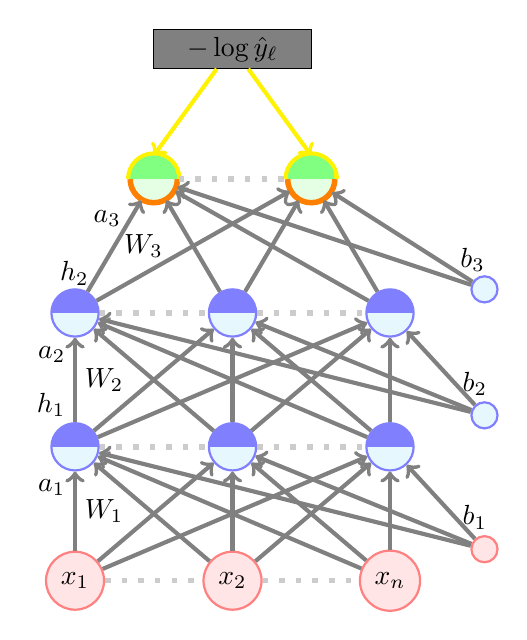
\begin{tikzpicture}


	\node [input_neuron] (neuron01) at (0,0) {$x_1$};
	\node [input_neuron] (neuron02) at (2,0){$x_2$};
	\node [input_neuron] (neuron03) at (4,0) {$x_n$};

	\node [bias_neuron] (neuron04) at (5.2,0.4) {};


	\node [hidden_neuron] (neuron11) at (0,1.7)  {};
	\node [hidden_neuron] (neuron12) at (2,1.7)  {};
	\node [hidden_neuron] (neuron13) at (4,1.7)  {};

	\node [bias_hidden_neuron] (neuron14) at (5.2,2.1) {};

	\begin{scope}
		\path[clip] (0,1.7) circle (3mm);
		\path[fill=blue!50] (-0.4,1.7) rectangle (0.3,2);
	\end{scope}
	\begin{scope}
		\path[clip] (2,1.7) circle (3mm);
		\path[fill=blue!50] (1.6,1.7) rectangle (2.3,2);
	\end{scope}
	\begin{scope}
		\path[clip] (4,1.7) circle (3mm);
		\path[fill=blue!50] (3.6,1.7) rectangle (4.3,2);
	\end{scope}


	\node [hidden_neuron] (neuron21) at (0,3.4)  {};
	\node [hidden_neuron] (neuron22) at (2,3.4)  {};
	\node [hidden_neuron] (neuron23) at (4,3.4)  {};

	\node [bias_hidden_neuron] (neuron24) at (5.2,3.7) {};


	\begin{scope}
		\path[clip] (0,3.4) circle (3mm);
		\path[fill=blue!50] (-0.4,3.4) rectangle (0.4,3.7);
	\end{scope}
	\begin{scope}
		\path[clip] (2,3.4) circle (3mm);
		\path[fill=blue!50] (1.6,3.4) rectangle (2.4,3.7);
	\end{scope}
	\begin{scope}
		\path[clip] (4,3.4) circle (3mm);
		\path[fill=blue!50] (3.6,3.4) rectangle (4.4,3.7);
	\end{scope}


	\node [output_neuron] (neuron31) at (1,5.1)  {};
	\node [output_neuron] (neuron32) at (3,5.1)  {};
	\draw [fill=gray] (1, 7) rectangle (3, 6.5) node[pos=0.5] {$-\log\hat{y}_\ell$};
	\draw [yellow,line width=1.5pt,  ->] (1.8, 6.5) -- (1, 5.4);
	\draw [yellow, line width=1.5pt, ->]  (2.2, 6.5) -- (3, 5.4);
	\draw [yellow, line width = 3] (1.3,5.1) arc (0:180:3mm) {};
	\draw [yellow, line width = 3] (3.3,5.1) arc (0:180:3mm) {};
	\draw[orange, line width = 2] (0.7, 5.1) arc (180:360:3mm){};
	\draw[orange, line width = 2] (2.7, 5.1) arc (180:360:3mm){};


	\begin{scope}
		\path[clip] (1,5.1) circle (3mm);
		\path[fill=green!50] (0.6,5.1) rectangle (1.3,5.4);
	\end{scope}
	\begin{scope}
		\path[clip] (3,5.1) circle (3mm);
		\path[fill=green!50] (2.6,5.1) rectangle (3.3,5.4);
	\end{scope}

	\draw[white,->] (neuron01) -- (neuron11) node[black,pos=.5,right]  {$W_{1}$} node[black,pos=0.8,left] {$a_{1}$};

	\draw[white,->] (neuron11) -- (neuron21) node[black,pos=.5,right] {$W_{2}$} node[black,pos=0.8,left] {$a_{2}$} node[black,pos=.2,left] {$h_{1}$};
	\draw[white,->] (neuron21) -- (neuron31) node[black,pos=.5,right] {$W_{3}$} node[black,pos=0.8,left] {$a_{3}$} node[black,pos=.2,left] {$h_{2}$};

	\draw[white,->] (neuron04) -- (neuron13) node[black,pos=0,right,above] {$b_1$};

	\draw[white,->] (neuron14) -- (neuron23) node[black,pos=0,right,above] {$b_2$};

	\draw[white,->] (neuron24) -- (neuron32) node[black,pos=0,right,above] {$b_3$};

	\draw[black!20,line width=2pt,loosely dotted] (neuron01) -- (neuron02);
	\draw[black!20,line width=2pt,loosely dotted] (neuron02) -- (neuron03);
	\draw[black!20,line width=2pt,loosely dotted] (neuron11) -- (neuron12);
	\draw[black!20,line width=2pt,loosely dotted] (neuron12) -- (neuron13);
	\draw[black!20,line width=2pt,loosely dotted] (neuron21) -- (neuron22);
	\draw[black!20,line width=2pt,loosely dotted] (neuron22) -- (neuron23);
	\draw[black!20,line width=2pt,loosely dotted] (neuron31) -- (neuron32);


	\foreach \from in {neuron01,neuron02,neuron03,neuron04}
	\foreach \to in {neuron11,neuron12,neuron13}
	\draw [black!50,line width=1.5pt,->] (\from) -- (\to);

	\foreach \from in {neuron11,neuron12,neuron13,neuron14}
	\foreach \to in {neuron21,neuron22,neuron23}
	\draw [black!50,line width=1.5pt,->] (\from) -- (\to);

	\foreach \from in {neuron21,neuron22,neuron23,neuron24}
	\foreach \to in {neuron31,neuron32}
	\draw [black!50,line width=1.5pt,->] (\from) -- (\to);


\end{tikzpicture}

    \end{overlayarea}
  \end{columns}
\end{frame}

%Slide 29
\begin{frame}
  \begin{columns}
    \column{0.6\textwidth}
    \begin{overlayarea}{\textwidth}{\textheight}
      \vspace{-0.5cm}
      \small{
        \begin{align*}
          \visible<1->{
            \frac{\partial}{\partial a_{Li} } - \log \hat{y}_{\ell}
            & =}
          \visible<2->{
            \frac{-1}{\hat{y}_{\ell}}
            \frac{\partial}{\partial a_{Li}} \hat{y}_{\ell}} \\
          \visible<3->{
            & = \frac{-1}{\hat{y}_{\ell}}
            \frac{\partial}{\partial a_{Li}} softmax(\mathbf{a}_{L})_{\ell}} \\
          \visible<4->{
            & = \frac{-1}{\hat{y}_{\ell}} \frac{\partial}{\partial a_{Li}}
            \frac{\exp(\mathbf{a}_{L})_{\ell}}{\sum_{i'} \exp(\mathbf{a}_{L})_{\ell}}} \\
          \visible<6->{
            & = \frac{-1}{\hat{y}_{\ell}}
            \Bigg(
            \frac{\frac{\partial}
              {\partial a_{Li}} \exp(\mathbf{a}_{L})_{\ell}}
            {\sum_{i'} \exp(\mathbf{a}_{L})_{i'}}
            -
            \frac
                {\exp(\mathbf{a}_{L})_{\ell}\Big(\frac{\partial}
              {\partial a_{Li}}
              \sum_{i'} \exp(\mathbf{a}_{L})_{i'}
              \Big)}
                {(\sum_{i'} (\exp(\mathbf{a}_{L})_{i'})^2}
            \Bigg) } \\
          \visible<7->{
            & = \frac{-1}{\hat{y}_{\ell}}
            \Bigg(
            \frac{\mathbbm{1}_{(\ell = i)} \exp(\mathbf{a}_{L})_{\ell}}
            {\sum_{i'} \exp(\mathbf{a}_{L})_{i'}}
            -
            \frac{\exp(\mathbf{a}_{L})_{\ell}}
            {\sum_{i'} \exp(\mathbf{a}_{L})_{i'}}
            \frac{\exp(\mathbf{a}_{L})_i}
            {\sum_{i'} \exp(\mathbf{a}_{L})_{i'}}
            \Bigg)} \\
          \visible<8->{
            & = \frac{-1}{\hat{y}_{\ell}}
            \bigg(
            \mathbbm{1}_{(\ell = i)} softmax(\mathbf{a}_{L})_{\ell}
            -
            softmax(\mathbf{a}_{L})_{\ell} softmax(\mathbf{a}_{L})_{i}
            \bigg)} \\
          \visible<9->{
            & = \frac{-1}{\hat{y}_{\ell}}
            \big(
            \mathbbm{1}_{(\ell = i)} \hat{y}_{\ell}
            -
            \hat{y}_{\ell} \hat{y}_i
            \big) } \\
          \visible<10->{
            & = -\big(
            \mathbbm{1}_{(\ell = i)}
            -
            \hat{y}_i
            \big)}
        \end{align*}
      }
    \end{overlayarea}

    \column{0.4\textwidth}
    \begin{overlayarea}{\textwidth}{\textheight}
      \visible<5->{
        $$
          \frac{\partial \frac{g(x)}{h(x)}}{\partial x}
          =
          \frac{\partial g(x)}{\partial x}
          \frac{1}{h(x)}
          -
          \frac{g(x)}{{h(x)}^2}
          \frac{\partial h(x)}{\partial x}
        $$
      }
    \end{overlayarea}
  \end{columns}
\end{frame}

%Slide 30
\begin{frame}
  \begin{columns}
    \column{0.62\textwidth}
    \begin{overlayarea}{\textwidth}{\textheight}
      So far we have derived the partial derivative w.r.t. the $i$-th element of $\mathbf{a}_{L}$
      \begin{equation*}
        \hspace{-2cm}\frac{\partial \mathscr{L}(\theta)}{\partial a_{L,i}} =
        - (\mathbbm{1}_{\ell = i} - \hat{y}_{i})
      \end{equation*}
      We can now write the gradient w.r.t. the vector $\mathbf{a}_{L}$

      \vspace{0.42cm}
      \begin{itemize}
        \justifying
        \item[]<2-> $\mathbf{\nabla_{a_{L}}} \mathscr{L}(\theta) \visible<3->{ =
                \begin{bmatrix}
                  \visible<3->{\frac{\partial \mathscr{L}(\theta)}{\partial a_{L1}}}   \\
                  \visible<4->{\vdots}                                              \\
                  \visible<5->{\frac{\partial \mathscr{L}(\theta)}{\partial a_{Lk}}} \\
                \end{bmatrix} }
              \visible<6->{ = \begin{bmatrix}
                  \visible<7->{ - (\mathbbm{1}_{\ell = 1} - \hat{y}_1)}       \\
                  \visible<8->{- (\mathbbm{1}_{\ell = 2} - \hat{y}_2)}        \\
                  \visible<9->{\vdots}                                     \\
                  \visible<10->{- (\mathbbm{1}_{\ell = k} - \hat{y}_{k})} \\
                \end{bmatrix} }$
        \item[]<11-> $\hspace{1cm}= - (\mathbf{e}(\ell) - \hat{y})$
      \end{itemize}
    \end{overlayarea}
    \column{0.38\textwidth}
    \begin{overlayarea}{\textwidth}{\textheight}
      \makebox[\textwidth][c]{\usebox{\nnoutputtwocontent}}
      % \hspace{-0.1in}
\tikzstyle{input_neuron}=[circle,draw=red!50,fill=red!10,thick,minimum size=5mm]
\tikzstyle{hidden_neuron}=[circle,draw=blue!50,fill=cyan!10,thick,minimum size=6mm]
\tikzstyle{output_neuron}=[circle,draw=green!50,fill=green!10,thick,minimum size=6mm]
\tikzstyle{bias_neuron}=[circle,draw=red!50,fill=red!10,thick,minimum size=2mm]
\tikzstyle{bias_hidden_neuron}=[circle,draw=blue!50,fill=cyan!10,thick,minimum size=2mm]

\tikzstyle{input}=[circle,draw=black!50,fill=black!20,thick,minimum size=6mm]

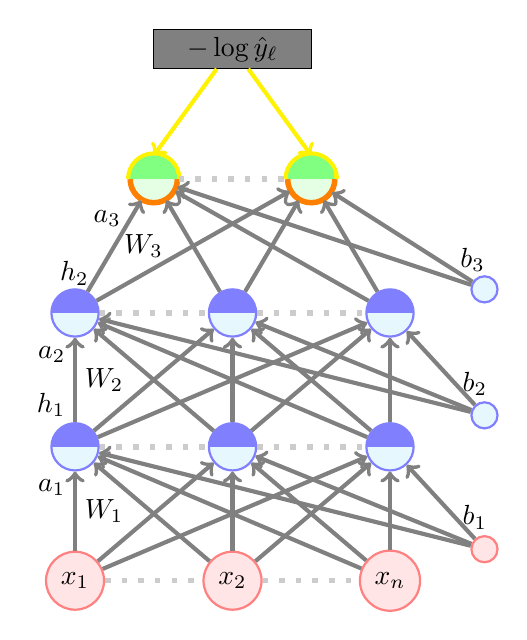
\begin{tikzpicture}


	\node [input_neuron] (neuron01) at (0,0) {$x_1$};
	\node [input_neuron] (neuron02) at (2,0){$x_2$};
	\node [input_neuron] (neuron03) at (4,0) {$x_n$};

	\node [bias_neuron] (neuron04) at (5.2,0.4) {};


	\node [hidden_neuron] (neuron11) at (0,1.7)  {};
	\node [hidden_neuron] (neuron12) at (2,1.7)  {};
	\node [hidden_neuron] (neuron13) at (4,1.7)  {};

	\node [bias_hidden_neuron] (neuron14) at (5.2,2.1) {};

	\begin{scope}
		\path[clip] (0,1.7) circle (3mm);
		\path[fill=blue!50] (-0.4,1.7) rectangle (0.3,2);
	\end{scope}
	\begin{scope}
		\path[clip] (2,1.7) circle (3mm);
		\path[fill=blue!50] (1.6,1.7) rectangle (2.3,2);
	\end{scope}
	\begin{scope}
		\path[clip] (4,1.7) circle (3mm);
		\path[fill=blue!50] (3.6,1.7) rectangle (4.3,2);
	\end{scope}


	\node [hidden_neuron] (neuron21) at (0,3.4)  {};
	\node [hidden_neuron] (neuron22) at (2,3.4)  {};
	\node [hidden_neuron] (neuron23) at (4,3.4)  {};

	\node [bias_hidden_neuron] (neuron24) at (5.2,3.7) {};


	\begin{scope}
		\path[clip] (0,3.4) circle (3mm);
		\path[fill=blue!50] (-0.4,3.4) rectangle (0.4,3.7);
	\end{scope}
	\begin{scope}
		\path[clip] (2,3.4) circle (3mm);
		\path[fill=blue!50] (1.6,3.4) rectangle (2.4,3.7);
	\end{scope}
	\begin{scope}
		\path[clip] (4,3.4) circle (3mm);
		\path[fill=blue!50] (3.6,3.4) rectangle (4.4,3.7);
	\end{scope}


	\node [output_neuron] (neuron31) at (1,5.1)  {};
	\node [output_neuron] (neuron32) at (3,5.1)  {};
	\draw [fill=gray] (1, 7) rectangle (3, 6.5) node[pos=0.5] {$-\log\hat{y}_\ell$};
	\draw [yellow,line width=1.5pt,  ->] (1.8, 6.5) -- (1, 5.4);
	\draw [yellow, line width=1.5pt, ->]  (2.2, 6.5) -- (3, 5.4);
	\draw [yellow, line width = 3] (1.3,5.1) arc (0:180:3mm) {};
	\draw [yellow, line width = 3] (3.3,5.1) arc (0:180:3mm) {};
	\draw[orange, line width = 2] (0.7, 5.1) arc (180:360:3mm){};
	\draw[orange, line width = 2] (2.7, 5.1) arc (180:360:3mm){};


	\begin{scope}
		\path[clip] (1,5.1) circle (3mm);
		\path[fill=green!50] (0.6,5.1) rectangle (1.3,5.4);
	\end{scope}
	\begin{scope}
		\path[clip] (3,5.1) circle (3mm);
		\path[fill=green!50] (2.6,5.1) rectangle (3.3,5.4);
	\end{scope}

	\draw[white,->] (neuron01) -- (neuron11) node[black,pos=.5,right]  {$W_{1}$} node[black,pos=0.8,left] {$a_{1}$};

	\draw[white,->] (neuron11) -- (neuron21) node[black,pos=.5,right] {$W_{2}$} node[black,pos=0.8,left] {$a_{2}$} node[black,pos=.2,left] {$h_{1}$};
	\draw[white,->] (neuron21) -- (neuron31) node[black,pos=.5,right] {$W_{3}$} node[black,pos=0.8,left] {$a_{3}$} node[black,pos=.2,left] {$h_{2}$};

	\draw[white,->] (neuron04) -- (neuron13) node[black,pos=0,right,above] {$b_1$};

	\draw[white,->] (neuron14) -- (neuron23) node[black,pos=0,right,above] {$b_2$};

	\draw[white,->] (neuron24) -- (neuron32) node[black,pos=0,right,above] {$b_3$};

	\draw[black!20,line width=2pt,loosely dotted] (neuron01) -- (neuron02);
	\draw[black!20,line width=2pt,loosely dotted] (neuron02) -- (neuron03);
	\draw[black!20,line width=2pt,loosely dotted] (neuron11) -- (neuron12);
	\draw[black!20,line width=2pt,loosely dotted] (neuron12) -- (neuron13);
	\draw[black!20,line width=2pt,loosely dotted] (neuron21) -- (neuron22);
	\draw[black!20,line width=2pt,loosely dotted] (neuron22) -- (neuron23);
	\draw[black!20,line width=2pt,loosely dotted] (neuron31) -- (neuron32);


	\foreach \from in {neuron01,neuron02,neuron03,neuron04}
	\foreach \to in {neuron11,neuron12,neuron13}
	\draw [black!50,line width=1.5pt,->] (\from) -- (\to);

	\foreach \from in {neuron11,neuron12,neuron13,neuron14}
	\foreach \to in {neuron21,neuron22,neuron23}
	\draw [black!50,line width=1.5pt,->] (\from) -- (\to);

	\foreach \from in {neuron21,neuron22,neuron23,neuron24}
	\foreach \to in {neuron31,neuron32}
	\draw [black!50,line width=1.5pt,->] (\from) -- (\to);


\end{tikzpicture}

    \end{overlayarea}
  \end{columns}
\end{frame}